\documentclass[12pt]{article}

% a template that a friend gave, it's worked well enough for me
% i have added some packages and stuff that have proved useful

\usepackage{fancyhdr}
\usepackage{tipa}
\usepackage{fontspec}
\usepackage{amsfonts}
\usepackage{enumitem}
\usepackage[margin=1in]{geometry}
\usepackage{graphicx}
\usepackage{float}
\usepackage{amsmath}
\usepackage{braket}
\usepackage{amssymb}
\usepackage{booktabs}
\usepackage{hyperref}
\usepackage{mathtools}
\usepackage{xcolor}
\usepackage{float}
\usepackage{algpseudocodex}
\usepackage{titlesec}
\usepackage{bbm}

\pagestyle{fancy}
\fancyhf{} % sets both header and footer to nothing
\lhead{Kevin Sheng}
\setmainfont{Comic Neue}
\renewcommand{\headrulewidth}{1pt}
\setlength{\headheight}{0.75in}
\setlength{\oddsidemargin}{0in}
\setlength{\evensidemargin}{0in}
\setlength{\voffset}{-.5in}
\setlength{\headsep}{10pt}
\setlength{\textwidth}{6.5in}
\setlength{\headwidth}{6.5in}
\setlength{\textheight}{8in}
\renewcommand{\headrulewidth}{0.5pt}
\renewcommand{\footrulewidth}{0.3pt}
\setlength{\textwidth}{6.5in}
\usepackage{setspace}
\usepackage{multicol}
\usepackage{float}
\setlength{\columnsep}{1cm}
\setlength\parindent{24pt}
\usepackage [english]{babel}
\usepackage [autostyle, english = american]{csquotes}
\MakeOuterQuote{"}

\setlength{\parskip}{6pt}
\setlength{\parindent}{0pt}

\titlespacing\section{0pt}{12pt plus 4pt minus 2pt}{0pt plus 2pt minus 2pt}
\titlespacing\subsection{0pt}{12pt plus 4pt minus 2pt}{0pt plus 2pt minus 2pt}
\titlespacing\subsubsection{0pt}{12pt plus 4pt minus 2pt}{0pt plus 2pt minus 2pt}

\hypersetup{colorlinks=true, urlcolor=blue}

\newcommand{\correction}[1]{\textcolor{red}{#1}}


\begin{document}
\section{Textbook}\label{sec:textbook}
\begin{itemize}
    \item[2.4.3] \textbf{Base case $n=1$:} \[1(1!)=(1+1)!-1\]
        Our inductive hypothesis is the following:
        \[\sum_{i=1}^n i(i!) = (n+1)!-1\]
        \textbf{Inductive step:}
        Given our inductive hypothesis, we must prove
        \[\sum_{i=1}^{n+1} i(i!) = (n+2)!-1\]
        To do this, we start from our inductive hypothesis and add $(n+1)(n+1)!$ to both sides.
        \begin{align*}
            \sum_{i=1}^n i(i!) + (n+1)(n+1)! & = (n+1)!-1 + (n+1)(n+1)! \\
            \sum_{i=1}^{n+1} i(i!)           & = (n+2)(n+1)!-1          \\
            \sum_{i=1}^{n+1} i(i!)           & = (n+2)!-1 \quad \square
        \end{align*}
    \item[2.4.6] \textbf{Base case $n=1$:}
        \[1^3=\left(\frac{1 \cdot 2}{2}\right)^2 \rightarrow \sum_{i=1}^n i^3 = \left(\frac{n(n+1)}{2}\right)^2\]
        \textbf{Inductive step:}
        We are to prove
        \[\sum_{i=1}^{n+1} i^3 = \left(\frac{(n+1)(n+2)}{2}\right)^2\]
        As in the previous problem, we start from our hypothesis and add $(n+1)^3$ to both sides.
        \begin{align*}
            \sum_{i=1}^n i^3 + (n+1)^3 & = \left(\frac{n(n+1)}{2}\right)^2 + (n+1)^3         \\
            \sum_{i=1}^{n+1} i^3       & = (n+1)^2\left(\frac{n^2}{4}+{n+1}\right)           \\
                                       & = (n+1)^2 \cdot \frac{(n+2)^2}{4}                   \\
                                       & = \left(\frac{(n+1)(n+2)}{2}\right)^2 \quad \square
        \end{align*}
    \item[3.1.18] $f(n)=n^2-1$ is not injective, as $f(1)=f(-1)=0$.
    It's not surjective either, since there's no value of $n$ s.t. $f(n)=-5$.
    This is because $n^2 \ge 0$, so $f(n) \ge 1$.
    \item[3.1.21] $f(n)=2n$ is injective, since if $x \ne y$, $f(x)=2x \ne 2y =f(y)$.
    However, it's not surjective, since there's no $n$ s.t. $f(n)=1$.
    The only solution to $2n=1$ lies in the rationals, which is outside the domain.
    \item[3.1.28] $f(m,n)=m+n+2$ is not injective, since $f(0,0)=f(1,-1)=2$.
    It is surjective, though, since for any $x \in \mathbb{Z}$ I know that $f(0,x-2)=0+x-2+2=x$.
\end{itemize}

\pagebreak

\section{Handout}\label{sec:handout}
\begin{itemize}
    \item[A1] \textbf{Base case $n=1$:} \[x^0=\frac{x-1}{x-1} \rightarrow \sum_{i=0}^{n-1} x^i=\frac{x^n-1}{x-1}\]
        \textbf{Inductive step:} \begin{align*}
            \sum_{i=0}^{n-1} x^i + x^n & = \frac{x^n-1}{x-1}+x^n             \\
            \sum_{i=0}^{n} x^i         & = \frac{x^n-1+x^{n+1}-x^n}{x-1}     \\
                                       & = \frac{x^{n+1}-1}{x-1}\quad\square
        \end{align*}
    \item[A2] \begin{enumerate}[label=\alph*]
            \item Since $g$ is injective, we know that $x \ne y \rightarrow g(x) \ne g(y)$.
                  Given that $f$ is also injective, we can say that $g(x) \ne g(y) \rightarrow f(g(x)) \ne f(g(y))$,
                  and thus $f \circ g$ is injective. $\square$
            \item Since $g$ is surjective, we know that $\forall z \in Z\ \exists y \in Y: g(y)=z$.
                  Applying the same logic to $f$, we have $\forall y \in Y\ \exists x \in X: f(x)=y$.
                  Linking these two relations, we have $\forall z \in Z\ \exists x \in X: g(f(x))=z$,
                  meaning that $g \circ f$ is surjective. $\square$
            \item This follows naturally from the first two propositions, since being bijective
                  is equivalent to being both surjective and injective, and we've just proved that $f$ and $g$ having these properties
                  means that $g \circ f$ also has them.
        \end{enumerate}
    \item[A3] We know that $f$ is both injective and surjective, and we have to show $\exists f^{-1}$ with the same properties.

        Since the domain of $f$ is the same as the range of $f^{-1}$, we know that $f^{-1}$ is surjective and can output any value of $X$. \\
        Also, since for any $x \in X$ can only have one output, if $f^{-1}(y)=f^{-1}(y')$ then $y=y'$, and thus $f^{-1}$ is also injective.
    \item[A4] \begin{enumerate}[label=\alph*]
            \item $f(x)=\sqrt{x}$ is injective but not surjective, since it only takes on positive values.
            \item Let $f(x, y)$ be the distance one has to walk on the given spiral from $(0, 0)$ to get to $(x, y)$.
                  For example, $f(1, 1)=2$ and $f(-1, 1)=4$.
                  \begin{center}
                      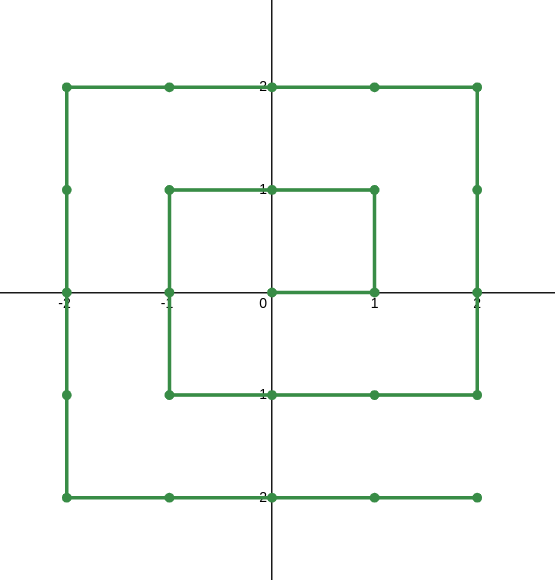
\includegraphics[width=5cm]{img/spiral} \\
                      \small{A diagram of the first few points of this spiral}
                  \end{center}
            \item $f(x)=(x-1)^2(x-2)$ takes on all values in $\mathbb{R}$, but $f(1)=f(2)=0$, so it's not injective.
        \end{enumerate}
\end{itemize}
\end{document}